\section{Extensions}
\label{sec:extensions}

  \subsection{Markov Model}
  \label{sec:markov_model}

  \subsection{BoW + NN}
  \label{sec:bow_nn}

  \subsection{Grid Searching}
  \label{sec:grid_search}

    \subsubsection{RNN}
    \label{sec:rnn_grid_search}

    \subsubsection{DNN}
    \label{sec:dnn_grid_search}

    \subsection{Ensemble}
    \label{sec:ensemble}

    \subsection{kPCA}
    \label{sec:kpca}
    An attempt was made to use kernel principal component analysis (kPCA) to help to produce more separable data. To do this a kPCA was used on a Count Vectorizer and a Term Frequency – Inverse Document Frequency Vectorizer.
    
    \begin{figure}[h]
\centering
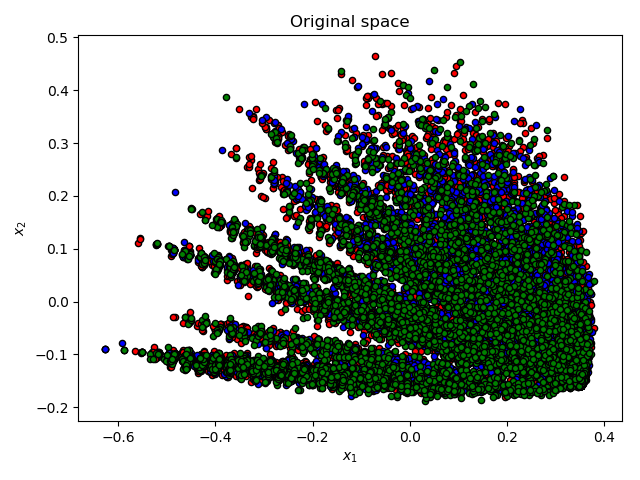
\includegraphics[width=\columnwidth]{Figures/Extensions/kPCALemmaRBF.png}
\caption{kPCA performed on a Lemma Count Vectorizer using RBF kernel and a gamma of 0.04}
\label{fig:balance}
\end{figure}
    
    
    
  
